\documentclass[10pt]{article}

\usepackage{tmlr}
% Camera-ready only: \usepackage[accepted]{tmlr}
% Preprint without a TMLR footer: \usepackage[preprint]{tmlr}

%%%%% NEW MATH DEFINITIONS %%%%%

\usepackage{amsmath,amsfonts,bm}

% Mark sections of captions for referring to divisions of figures
\newcommand{\figleft}{{\em (Left)}}
\newcommand{\figcenter}{{\em (Center)}}
\newcommand{\figright}{{\em (Right)}}
\newcommand{\figtop}{{\em (Top)}}
\newcommand{\figbottom}{{\em (Bottom)}}
\newcommand{\captiona}{{\em (a)}}
\newcommand{\captionb}{{\em (b)}}
\newcommand{\captionc}{{\em (c)}}
\newcommand{\captiond}{{\em (d)}}

% Highlight a newly defined term
\newcommand{\newterm}[1]{{\bf #1}}


% Figure reference, lower-case.
\def\figref#1{figure~\ref{#1}}
% Figure reference, capital. For start of sentence
\def\Figref#1{Figure~\ref{#1}}
\def\twofigref#1#2{figures \ref{#1} and \ref{#2}}
\def\quadfigref#1#2#3#4{figures \ref{#1}, \ref{#2}, \ref{#3} and \ref{#4}}
% Section reference, lower-case.
\def\secref#1{section~\ref{#1}}
% Section reference, capital.
\def\Secref#1{Section~\ref{#1}}
% Reference to two sections.
\def\twosecrefs#1#2{sections \ref{#1} and \ref{#2}}
% Reference to three sections.
\def\secrefs#1#2#3{sections \ref{#1}, \ref{#2} and \ref{#3}}
% Reference to an equation, lower-case.
\def\eqref#1{equation~\ref{#1}}
% Reference to an equation, upper case
\def\Eqref#1{Equation~\ref{#1}}
% A raw reference to an equation---avoid using if possible
\def\plaineqref#1{\ref{#1}}
% Reference to a chapter, lower-case.
\def\chapref#1{chapter~\ref{#1}}
% Reference to an equation, upper case.
\def\Chapref#1{Chapter~\ref{#1}}
% Reference to a range of chapters
\def\rangechapref#1#2{chapters\ref{#1}--\ref{#2}}
% Reference to an algorithm, lower-case.
\def\algref#1{algorithm~\ref{#1}}
% Reference to an algorithm, upper case.
\def\Algref#1{Algorithm~\ref{#1}}
\def\twoalgref#1#2{algorithms \ref{#1} and \ref{#2}}
\def\Twoalgref#1#2{Algorithms \ref{#1} and \ref{#2}}
% Reference to a part, lower case
\def\partref#1{part~\ref{#1}}
% Reference to a part, upper case
\def\Partref#1{Part~\ref{#1}}
\def\twopartref#1#2{parts \ref{#1} and \ref{#2}}

\def\ceil#1{\lceil #1 \rceil}
\def\floor#1{\lfloor #1 \rfloor}
\def\1{\bm{1}}
\newcommand{\train}{\mathcal{D}}
\newcommand{\valid}{\mathcal{D_{\mathrm{valid}}}}
\newcommand{\test}{\mathcal{D_{\mathrm{test}}}}

\def\eps{{\epsilon}}


% Random variables
\def\reta{{\textnormal{$\eta$}}}
\def\ra{{\textnormal{a}}}
\def\rb{{\textnormal{b}}}
\def\rc{{\textnormal{c}}}
\def\rd{{\textnormal{d}}}
\def\re{{\textnormal{e}}}
\def\rf{{\textnormal{f}}}
\def\rg{{\textnormal{g}}}
\def\rh{{\textnormal{h}}}
\def\ri{{\textnormal{i}}}
\def\rj{{\textnormal{j}}}
\def\rk{{\textnormal{k}}}
\def\rl{{\textnormal{l}}}
% rm is already a command, just don't name any random variables m
\def\rn{{\textnormal{n}}}
\def\ro{{\textnormal{o}}}
\def\rp{{\textnormal{p}}}
\def\rq{{\textnormal{q}}}
\def\rr{{\textnormal{r}}}
\def\rs{{\textnormal{s}}}
\def\rt{{\textnormal{t}}}
\def\ru{{\textnormal{u}}}
\def\rv{{\textnormal{v}}}
\def\rw{{\textnormal{w}}}
\def\rx{{\textnormal{x}}}
\def\ry{{\textnormal{y}}}
\def\rz{{\textnormal{z}}}

% Random vectors
\def\rvepsilon{{\mathbf{\epsilon}}}
\def\rvtheta{{\mathbf{\theta}}}
\def\rva{{\mathbf{a}}}
\def\rvb{{\mathbf{b}}}
\def\rvc{{\mathbf{c}}}
\def\rvd{{\mathbf{d}}}
\def\rve{{\mathbf{e}}}
\def\rvf{{\mathbf{f}}}
\def\rvg{{\mathbf{g}}}
\def\rvh{{\mathbf{h}}}
\def\rvu{{\mathbf{i}}}
\def\rvj{{\mathbf{j}}}
\def\rvk{{\mathbf{k}}}
\def\rvl{{\mathbf{l}}}
\def\rvm{{\mathbf{m}}}
\def\rvn{{\mathbf{n}}}
\def\rvo{{\mathbf{o}}}
\def\rvp{{\mathbf{p}}}
\def\rvq{{\mathbf{q}}}
\def\rvr{{\mathbf{r}}}
\def\rvs{{\mathbf{s}}}
\def\rvt{{\mathbf{t}}}
\def\rvu{{\mathbf{u}}}
\def\rvv{{\mathbf{v}}}
\def\rvw{{\mathbf{w}}}
\def\rvx{{\mathbf{x}}}
\def\rvy{{\mathbf{y}}}
\def\rvz{{\mathbf{z}}}

% Elements of random vectors
\def\erva{{\textnormal{a}}}
\def\ervb{{\textnormal{b}}}
\def\ervc{{\textnormal{c}}}
\def\ervd{{\textnormal{d}}}
\def\erve{{\textnormal{e}}}
\def\ervf{{\textnormal{f}}}
\def\ervg{{\textnormal{g}}}
\def\ervh{{\textnormal{h}}}
\def\ervi{{\textnormal{i}}}
\def\ervj{{\textnormal{j}}}
\def\ervk{{\textnormal{k}}}
\def\ervl{{\textnormal{l}}}
\def\ervm{{\textnormal{m}}}
\def\ervn{{\textnormal{n}}}
\def\ervo{{\textnormal{o}}}
\def\ervp{{\textnormal{p}}}
\def\ervq{{\textnormal{q}}}
\def\ervr{{\textnormal{r}}}
\def\ervs{{\textnormal{s}}}
\def\ervt{{\textnormal{t}}}
\def\ervu{{\textnormal{u}}}
\def\ervv{{\textnormal{v}}}
\def\ervw{{\textnormal{w}}}
\def\ervx{{\textnormal{x}}}
\def\ervy{{\textnormal{y}}}
\def\ervz{{\textnormal{z}}}

% Random matrices
\def\rmA{{\mathbf{A}}}
\def\rmB{{\mathbf{B}}}
\def\rmC{{\mathbf{C}}}
\def\rmD{{\mathbf{D}}}
\def\rmE{{\mathbf{E}}}
\def\rmF{{\mathbf{F}}}
\def\rmG{{\mathbf{G}}}
\def\rmH{{\mathbf{H}}}
\def\rmI{{\mathbf{I}}}
\def\rmJ{{\mathbf{J}}}
\def\rmK{{\mathbf{K}}}
\def\rmL{{\mathbf{L}}}
\def\rmM{{\mathbf{M}}}
\def\rmN{{\mathbf{N}}}
\def\rmO{{\mathbf{O}}}
\def\rmP{{\mathbf{P}}}
\def\rmQ{{\mathbf{Q}}}
\def\rmR{{\mathbf{R}}}
\def\rmS{{\mathbf{S}}}
\def\rmT{{\mathbf{T}}}
\def\rmU{{\mathbf{U}}}
\def\rmV{{\mathbf{V}}}
\def\rmW{{\mathbf{W}}}
\def\rmX{{\mathbf{X}}}
\def\rmY{{\mathbf{Y}}}
\def\rmZ{{\mathbf{Z}}}

% Elements of random matrices
\def\ermA{{\textnormal{A}}}
\def\ermB{{\textnormal{B}}}
\def\ermC{{\textnormal{C}}}
\def\ermD{{\textnormal{D}}}
\def\ermE{{\textnormal{E}}}
\def\ermF{{\textnormal{F}}}
\def\ermG{{\textnormal{G}}}
\def\ermH{{\textnormal{H}}}
\def\ermI{{\textnormal{I}}}
\def\ermJ{{\textnormal{J}}}
\def\ermK{{\textnormal{K}}}
\def\ermL{{\textnormal{L}}}
\def\ermM{{\textnormal{M}}}
\def\ermN{{\textnormal{N}}}
\def\ermO{{\textnormal{O}}}
\def\ermP{{\textnormal{P}}}
\def\ermQ{{\textnormal{Q}}}
\def\ermR{{\textnormal{R}}}
\def\ermS{{\textnormal{S}}}
\def\ermT{{\textnormal{T}}}
\def\ermU{{\textnormal{U}}}
\def\ermV{{\textnormal{V}}}
\def\ermW{{\textnormal{W}}}
\def\ermX{{\textnormal{X}}}
\def\ermY{{\textnormal{Y}}}
\def\ermZ{{\textnormal{Z}}}

% Vectors
\def\vzero{{\bm{0}}}
\def\vone{{\bm{1}}}
\def\vmu{{\bm{\mu}}}
\def\vtheta{{\bm{\theta}}}
\def\va{{\bm{a}}}
\def\vb{{\bm{b}}}
\def\vc{{\bm{c}}}
\def\vd{{\bm{d}}}
\def\ve{{\bm{e}}}
\def\vf{{\bm{f}}}
\def\vg{{\bm{g}}}
\def\vh{{\bm{h}}}
\def\vi{{\bm{i}}}
\def\vj{{\bm{j}}}
\def\vk{{\bm{k}}}
\def\vl{{\bm{l}}}
\def\vm{{\bm{m}}}
\def\vn{{\bm{n}}}
\def\vo{{\bm{o}}}
\def\vp{{\bm{p}}}
\def\vq{{\bm{q}}}
\def\vr{{\bm{r}}}
\def\vs{{\bm{s}}}
\def\vt{{\bm{t}}}
\def\vu{{\bm{u}}}
\def\vv{{\bm{v}}}
\def\vw{{\bm{w}}}
\def\vx{{\bm{x}}}
\def\vy{{\bm{y}}}
\def\vz{{\bm{z}}}

% Elements of vectors
\def\evalpha{{\alpha}}
\def\evbeta{{\beta}}
\def\evepsilon{{\epsilon}}
\def\evlambda{{\lambda}}
\def\evomega{{\omega}}
\def\evmu{{\mu}}
\def\evpsi{{\psi}}
\def\evsigma{{\sigma}}
\def\evtheta{{\theta}}
\def\eva{{a}}
\def\evb{{b}}
\def\evc{{c}}
\def\evd{{d}}
\def\eve{{e}}
\def\evf{{f}}
\def\evg{{g}}
\def\evh{{h}}
\def\evi{{i}}
\def\evj{{j}}
\def\evk{{k}}
\def\evl{{l}}
\def\evm{{m}}
\def\evn{{n}}
\def\evo{{o}}
\def\evp{{p}}
\def\evq{{q}}
\def\evr{{r}}
\def\evs{{s}}
\def\evt{{t}}
\def\evu{{u}}
\def\evv{{v}}
\def\evw{{w}}
\def\evx{{x}}
\def\evy{{y}}
\def\evz{{z}}

% Matrix
\def\mA{{\bm{A}}}
\def\mB{{\bm{B}}}
\def\mC{{\bm{C}}}
\def\mD{{\bm{D}}}
\def\mE{{\bm{E}}}
\def\mF{{\bm{F}}}
\def\mG{{\bm{G}}}
\def\mH{{\bm{H}}}
\def\mI{{\bm{I}}}
\def\mJ{{\bm{J}}}
\def\mK{{\bm{K}}}
\def\mL{{\bm{L}}}
\def\mM{{\bm{M}}}
\def\mN{{\bm{N}}}
\def\mO{{\bm{O}}}
\def\mP{{\bm{P}}}
\def\mQ{{\bm{Q}}}
\def\mR{{\bm{R}}}
\def\mS{{\bm{S}}}
\def\mT{{\bm{T}}}
\def\mU{{\bm{U}}}
\def\mV{{\bm{V}}}
\def\mW{{\bm{W}}}
\def\mX{{\bm{X}}}
\def\mY{{\bm{Y}}}
\def\mZ{{\bm{Z}}}
\def\mBeta{{\bm{\beta}}}
\def\mPhi{{\bm{\Phi}}}
\def\mLambda{{\bm{\Lambda}}}
\def\mSigma{{\bm{\Sigma}}}

% Tensor
\DeclareMathAlphabet{\mathsfit}{\encodingdefault}{\sfdefault}{m}{sl}
\SetMathAlphabet{\mathsfit}{bold}{\encodingdefault}{\sfdefault}{bx}{n}
\newcommand{\tens}[1]{\bm{\mathsfit{#1}}}
\def\tA{{\tens{A}}}
\def\tB{{\tens{B}}}
\def\tC{{\tens{C}}}
\def\tD{{\tens{D}}}
\def\tE{{\tens{E}}}
\def\tF{{\tens{F}}}
\def\tG{{\tens{G}}}
\def\tH{{\tens{H}}}
\def\tI{{\tens{I}}}
\def\tJ{{\tens{J}}}
\def\tK{{\tens{K}}}
\def\tL{{\tens{L}}}
\def\tM{{\tens{M}}}
\def\tN{{\tens{N}}}
\def\tO{{\tens{O}}}
\def\tP{{\tens{P}}}
\def\tQ{{\tens{Q}}}
\def\tR{{\tens{R}}}
\def\tS{{\tens{S}}}
\def\tT{{\tens{T}}}
\def\tU{{\tens{U}}}
\def\tV{{\tens{V}}}
\def\tW{{\tens{W}}}
\def\tX{{\tens{X}}}
\def\tY{{\tens{Y}}}
\def\tZ{{\tens{Z}}}


% Graph
\def\gA{{\mathcal{A}}}
\def\gB{{\mathcal{B}}}
\def\gC{{\mathcal{C}}}
\def\gD{{\mathcal{D}}}
\def\gE{{\mathcal{E}}}
\def\gF{{\mathcal{F}}}
\def\gG{{\mathcal{G}}}
\def\gH{{\mathcal{H}}}
\def\gI{{\mathcal{I}}}
\def\gJ{{\mathcal{J}}}
\def\gK{{\mathcal{K}}}
\def\gL{{\mathcal{L}}}
\def\gM{{\mathcal{M}}}
\def\gN{{\mathcal{N}}}
\def\gO{{\mathcal{O}}}
\def\gP{{\mathcal{P}}}
\def\gQ{{\mathcal{Q}}}
\def\gR{{\mathcal{R}}}
\def\gS{{\mathcal{S}}}
\def\gT{{\mathcal{T}}}
\def\gU{{\mathcal{U}}}
\def\gV{{\mathcal{V}}}
\def\gW{{\mathcal{W}}}
\def\gX{{\mathcal{X}}}
\def\gY{{\mathcal{Y}}}
\def\gZ{{\mathcal{Z}}}

% Sets
\def\sA{{\mathbb{A}}}
\def\sB{{\mathbb{B}}}
\def\sC{{\mathbb{C}}}
\def\sD{{\mathbb{D}}}
% Don't use a set called E, because this would be the same as our symbol
% for expectation.
\def\sF{{\mathbb{F}}}
\def\sG{{\mathbb{G}}}
\def\sH{{\mathbb{H}}}
\def\sI{{\mathbb{I}}}
\def\sJ{{\mathbb{J}}}
\def\sK{{\mathbb{K}}}
\def\sL{{\mathbb{L}}}
\def\sM{{\mathbb{M}}}
\def\sN{{\mathbb{N}}}
\def\sO{{\mathbb{O}}}
\def\sP{{\mathbb{P}}}
\def\sQ{{\mathbb{Q}}}
\def\sR{{\mathbb{R}}}
\def\sS{{\mathbb{S}}}
\def\sT{{\mathbb{T}}}
\def\sU{{\mathbb{U}}}
\def\sV{{\mathbb{V}}}
\def\sW{{\mathbb{W}}}
\def\sX{{\mathbb{X}}}
\def\sY{{\mathbb{Y}}}
\def\sZ{{\mathbb{Z}}}

% Entries of a matrix
\def\emLambda{{\Lambda}}
\def\emA{{A}}
\def\emB{{B}}
\def\emC{{C}}
\def\emD{{D}}
\def\emE{{E}}
\def\emF{{F}}
\def\emG{{G}}
\def\emH{{H}}
\def\emI{{I}}
\def\emJ{{J}}
\def\emK{{K}}
\def\emL{{L}}
\def\emM{{M}}
\def\emN{{N}}
\def\emO{{O}}
\def\emP{{P}}
\def\emQ{{Q}}
\def\emR{{R}}
\def\emS{{S}}
\def\emT{{T}}
\def\emU{{U}}
\def\emV{{V}}
\def\emW{{W}}
\def\emX{{X}}
\def\emY{{Y}}
\def\emZ{{Z}}
\def\emSigma{{\Sigma}}

% entries of a tensor
% Same font as tensor, without \bm wrapper
\newcommand{\etens}[1]{\mathsfit{#1}}
\def\etLambda{{\etens{\Lambda}}}
\def\etA{{\etens{A}}}
\def\etB{{\etens{B}}}
\def\etC{{\etens{C}}}
\def\etD{{\etens{D}}}
\def\etE{{\etens{E}}}
\def\etF{{\etens{F}}}
\def\etG{{\etens{G}}}
\def\etH{{\etens{H}}}
\def\etI{{\etens{I}}}
\def\etJ{{\etens{J}}}
\def\etK{{\etens{K}}}
\def\etL{{\etens{L}}}
\def\etM{{\etens{M}}}
\def\etN{{\etens{N}}}
\def\etO{{\etens{O}}}
\def\etP{{\etens{P}}}
\def\etQ{{\etens{Q}}}
\def\etR{{\etens{R}}}
\def\etS{{\etens{S}}}
\def\etT{{\etens{T}}}
\def\etU{{\etens{U}}}
\def\etV{{\etens{V}}}
\def\etW{{\etens{W}}}
\def\etX{{\etens{X}}}
\def\etY{{\etens{Y}}}
\def\etZ{{\etens{Z}}}

% The true underlying data generating distribution
\newcommand{\pdata}{p_{\rm{data}}}
% The empirical distribution defined by the training set
\newcommand{\ptrain}{\hat{p}_{\rm{data}}}
\newcommand{\Ptrain}{\hat{P}_{\rm{data}}}
% The model distribution
\newcommand{\pmodel}{p_{\rm{model}}}
\newcommand{\Pmodel}{P_{\rm{model}}}
\newcommand{\ptildemodel}{\tilde{p}_{\rm{model}}}
% Stochastic autoencoder distributions
\newcommand{\pencode}{p_{\rm{encoder}}}
\newcommand{\pdecode}{p_{\rm{decoder}}}
\newcommand{\precons}{p_{\rm{reconstruct}}}

\newcommand{\laplace}{\mathrm{Laplace}} % Laplace distribution

\newcommand{\E}{\mathbb{E}}
\newcommand{\Ls}{\mathcal{L}}
\newcommand{\R}{\mathbb{R}}
\newcommand{\emp}{\tilde{p}}
\newcommand{\lr}{\alpha}
\newcommand{\reg}{\lambda}
\newcommand{\rect}{\mathrm{rectifier}}
\newcommand{\softmax}{\mathrm{softmax}}
\newcommand{\sigmoid}{\sigma}
\newcommand{\softplus}{\zeta}
\newcommand{\KL}{D_{\mathrm{KL}}}
\newcommand{\Var}{\mathrm{Var}}
\newcommand{\standarderror}{\mathrm{SE}}
\newcommand{\Cov}{\mathrm{Cov}}
% Wolfram Mathworld says $L^2$ is for function spaces and $\ell^2$ is for vectors
% But then they seem to use $L^2$ for vectors throughout the site, and so does
% wikipedia.
\newcommand{\normlzero}{L^0}
\newcommand{\normlone}{L^1}
\newcommand{\normltwo}{L^2}
\newcommand{\normlp}{L^p}
\newcommand{\normmax}{L^\infty}

\newcommand{\parents}{Pa} % See usage in notation.tex. Chosen to match Daphne's book.

\DeclareMathOperator*{\argmax}{arg\,max}
\DeclareMathOperator*{\argmin}{arg\,min}

\DeclareMathOperator{\sign}{sign}
\DeclareMathOperator{\Tr}{Tr}
\let\ab\allowbreak


\usepackage{hyperref}
\usepackage{url}
\usepackage{booktabs}
\usepackage{amsfonts}
\usepackage{nicefrac}
\usepackage{microtype}
\usepackage{xcolor}
\usepackage{graphicx}

\title{Same-drug continuity, not a target profile: a negative result for trial adverse-event transfer}

% Hidden while tmlr.sty is loaded without [accepted] or [preprint].
\author{\name{Anonymous} \email{anonymous@example.com} \\
\addr{Anonymized for double-blind review}}

\def\month{00}
\def\year{0000}
\def\openreview{\url{https://openreview.net/forum?id=XXXX}}

\begin{document}

\maketitle

\begin{abstract}
Biological features are often added to chemical fingerprints in the hope that they survive a change of population.
On smoothed adverse-event incidence from ClinicalTrials.gov, that hope fails once evaluation is restricted to structures absent from the adult-trial rows.
The confirmatory task is adult-only-trial to pediatric-only-trial transfer of a reporting rate, not clinical pediatric toxicity and not an in-vitro assay.
A ridge model with pre-specified penalty $10$, Morgan fingerprints, and RDKit descriptors has macro Spearman $0.0314$ on twelve endpoints frozen before fitting.
Early fusion with a $15$-target ChEMBL profile (mean missingness $0.9242$) reaches $0.0339$.
The difference is $0.0025$ ($95\%$ CI $-0.0106$ to $0.0149$).
Against five training-row permutations of the profile the difference is $0.0031$ ($95\%$ CI $-0.0143$ to $0.0213$).
A coverage gate differs from chemistry by $-0.0007$ ($95\%$ CI $-0.0029$ to $0.0014$) and raises the negative-transfer count from $5$ endpoints to $7$.
The same chemistry model scores $0.1923$ on structures that do appear in both trial sets.
The historical appearance of a pediatric signal is largely that overlap.
A later pre-registered phase, with other fusion rules and a small multitask network, also found no arm whose intervals against chemistry and against a permutation control both lay above $0$.
The null is narrow: it concerns this sparse channel and this label.
\end{abstract}

\section{Introduction: expected versus observed}
\label{sec:intro}

A recurring expectation in molecular machine learning is that a biological representation should help when chemistry alone is asked to move to a new set of compounds.
The desired improvement here was specific.
On pediatric-only-trial adverse-event incidence, early fusion of chemistry with a ChEMBL target profile, and a gate that trusts that fusion only when the profile is observed, should beat chemistry, and should beat chemistry plus a profile whose compound--target correspondence has been destroyed.
Negative transfer, in the sense of a source-trained multimodal score that ranks the target worse than the chemical score \citep{zhang2023negativetransfer}, should become less common under the gate.

What was observed is a null on all three pre-specified tests (Section~\ref{sec:results}).
The same chemical model looks much stronger on pediatric-trial rows whose structure was already present in an adult trial (macro Spearman $0.1923$) than on rows whose structure was not ($0.0314$).
% src: results/tables/slice_macro.csv structure_seen/chem 0.1923 and structure_unseen/chem 0.0314
An archived review of an earlier model on these tables already described an overall mean near $0.12$ as continuity of the shared structures rather than generalization.
% src: archive/prior_verdicts/pediatric_transfer_v3_independent_review.json, wording ``overall mean ~0.12''; not recomputed in this fit
This paper's contribution is to freeze the structure-unseen slice, the eligibility rule, and the three contrasts before fitting, and to report the failure with intervals.

Section~\ref{sec:problem} states the task.
Section~\ref{sec:protocol} states the approach that was expected to help.
Section~\ref{sec:results} states the null.
Section~\ref{sec:why} states why the expected gain did not appear.

\section{Related work}
\label{sec:related}

MoleculeNet popularized scaffold-aware evaluation of in-vitro toxicity models and included the Tox21 assay panel \citep{wu2018moleculenet,tice2013tox21}.
Extended-connectivity fingerprints \citep{rogers2010ecfp} and Bemis--Murcko frameworks \citep{bemis1996frameworks} are the chemical representation and the grouping used here.
The Chemical Checker showed that bioactivity signatures can extend similarity beyond structure \citep{duranfrigola2020chemicalchecker}.
Those signatures were not regenerated for this study: the generator did not import, and a data license was not established.
An archived Tox21 notebook, using a different model, reported pooled task-macro AUROC $0.8224$ for chemistry and $0.8254$ for chemistry plus nine signature spaces.
% src: reports/initial_audit.md Notebook 2 saved cell output; not recomputed
The difference of those two saved figures is $0.0030$.
% src: reports/initial_audit.md, 0.8254 minus 0.8224
That gap is prior exploratory context.
It is not a result of the fit below, and it is not a trial-incidence result.

ChEMBL is a public bioactivity resource \citep{zdrazil2024chembl}.
The matrix used for the confirmatory fit is a $15$-target profile inherited from an earlier adult-coverage filter, not a current full ChEMBL release.
The release identifier was not recorded with that vocabulary.
Correlation alignment (CORAL) is a transductive covariance-matching method that does not use target labels \citep{sun2016coral}.
It is reported only as an exploratory arm.
Ridge regression is the confirmatory estimator \citep{hoerl1970ridge}, fit with scikit-learn \citep{pedregosa2011sklearn}.
Tree models use the pre-specified sizes in the config, including XGBoost \citep{chen2016xgboost}, and do not choose the claim.

\section{Problem setup and task renaming}
\label{sec:problem}

\textbf{Problem.}
The biological task that the files can support is ranking of smoothed logit adverse-event incidence across drug structures.
The source domain is adult-only interventional trials (minimum age at least $18$).
The target domain is pediatric-only trials (maximum age at most $17$).
Mixed-age trials were already excluded by the upstream aggregate \citep{clinicaltrials}.
The label is $(a+0.5)/(n+1)$ and then the logit, where $a$ is the count affected and $n$ is the count at risk.
The loader checks that this recomputation matches the stored column.
The quantity is a trial-reporting construct.
It is entangled with indication, dose, schedule, and how completely a trial records events.
It is not a causal risk and not a developmental-toxicity call.

Calling the target ``pediatric toxicity'' would overstate the label.
Tox21 labels are in-vitro assay activities.
FAERS reporting fractions, used in earlier probes of $137$ and $46$ compounds, do not match either Tox21 or this incidence label, and this paper reports no performance number for them.
The renamed confirmatory task is adult-trial to pediatric-trial adverse-event incidence transfer.

The primary population is the pediatric-trial structures whose InChIKey \citep{heller2015inchi} is absent from every adult-trial row: $201$ structures, against $634$ structures present in both sets, out of $835$ pediatric-trial and $2{,}856$ adult-trial structures.
% src: results/tables/dataset_characteristics.csv
A pre-fit count found that $48$ of those $201$ still share a Bemis--Murcko scaffold with an adult structure.
% src: reports/experiment_log.md, measured before model fitting
Scaffold-unseen rows are a sensitivity slice, not the primary filter.

The target metric is the unweighted mean, across eligible endpoints, of Spearman rank correlation.
Accuracy is not used.
AUROC is not used on the logit incidence label.
A multimodal benefit required both of the following $95\%$ endpoint-bootstrap intervals to lie entirely above $0$: early fusion minus chemistry, and early fusion minus the mean of the permutation seeds.
A gate gain required the coverage-gate interval versus chemistry to lie entirely above $0$.
Separately, the gate reduces negative transfer only if it has strictly fewer endpoints with a negative delta than early fusion and its macro Spearman is at least chemistry minus $0.005$.
Intervals that include $0$ are not superiority claims.
Benjamini--Hochberg $q$-values are reported across the three tests \citep{benjamini1995fdr}.

\section{Data provenance}
\label{sec:data}

Chemistry is recomputed from SMILES: Morgan radius $2$, $2{,}048$ bits \citep{rogers2010ecfp}, plus $217$ RDKit descriptors \citep{rdkit}, with a parameter-free $\log(1+x)$ on two unbounded indices before any split.
The model matrix has $2{,}265$ chemistry columns after the training-fold filters.
% src: results/tables/dataset_characteristics.csv n_chem_features 2265
Twelve InChIKeys had conflicting SMILES; the mode was kept.
Standardization failures were $0$ on $3{,}057$ structures.
% src: reports/experiment_log.md
Median imputation, clipping, a variance filter, and scaling are fit on training rows only.

The biological channel is $15$ ChEMBL targets plus $15$ missingness indicators.
Mean missingness is $0.9242$, mean coverage is $0.0758$, and the fraction of structures with any observed target is $0.3811$.
% src: results/tables/representation_coverage.csv
Coverage is one minus mean target missingness.
The profile was not derived from the trial labels.
Chemical Checker signatures are absent; treating the code license of the generator as a data license would be a mistake.
The ChEMBL-derived matrix is not redistributed with this draft.

Endpoints need at least $200$ adult rows and at least $40$ structure-unseen rows.
That cutoff was fixed before the confirmatory fit.
It keeps $12$ of $15$ endpoints and drops congenital/developmental ($24$ unseen), hepatic ($32$), and renal ($34$).
% src: results/tables/endpoint_inclusion.csv
Per-endpoint unseen counts on the kept endpoints run from $49$ (cardiac) to $200$ (the two aggregate labels).

\section{Protocol}
\label{sec:protocol}

\textbf{Proposed approach.}
The hypothesis was that, where targets are measured, the profile carries information about adverse-event incidence that fingerprints miss, and that a gate
\[
\hat y = (1-g)\,\hat y_{\mathrm{chem}} + g\,\hat y_{\mathrm{early}},
\]
with $g$ equal to the fraction of the $15$ targets observed, would fall back to chemistry when the profile is empty and would therefore cut negative transfer.

The confirmatory estimator is ridge regression with penalty $10$, solver \texttt{lsqr}, not tuned on pediatric labels \citep{hoerl1970ridge}.
A nested penalty search exists in a full config and was not run.
Adult in-domain scores are five-fold GroupKFold on Bemis--Murcko scaffolds.
Fusion weights and isotonic maps are fit on those adult out-of-fold predictions only.
Permutation seeds are $101$, $202$, $303$, $404$, and $505$.
Each permutation shuffles training rows of the biological block and leaves test rows intact.
The endpoint-bootstrap uses $1{,}000$ resamples and seed $0$.
% src: results/tables/hyperparameters.csv
Random forest and XGBoost are robustness checks at $40$ trees.
Their adult out-of-fold loop is off in this run.
CORAL, after a source-fit principal-component projection of width $32$, and importance weighting see unlabeled pediatric chemistry \citep{sun2016coral}.
A target-only ridge reference uses labels on half of the structure-unseen compounds.
None of those three is a confirmatory test.
Adversarial and kernel alignment methods were not fit, because a fair tuning loop would have been tempted to use the transfer labels.

Leakage checks on the fit recorded disjoint adult folds, a permutation that preserves the training multiset, preprocessing statistics that ignore the held-out fold, and a structure-unseen mask with no adult overlap.
The wall clock of the confirmatory process was $626$ seconds on four threads, with features already cached, covering $15$ trial endpoints and a separate Tox21 logistic arm.
% src: results/tables/compute_runtime.csv

\section{Observed outcome}
\label{sec:results}

On the structure-unseen slice the macro Spearman values are $0.0314$ (chemistry), $0.0339$ (early fusion), and $0.0308$ (coverage gate).
% src: reports/results.md, also results/metrics/primary_claims.json
Table~\ref{tab:primary} is the confirmatory family.
All three intervals include $0$.
The Benjamini--Hochberg $q$-values are $0.7600$, $0.7600$, and $0.7600$.
A Wilcoxon signed-rank $p$-value on the twelve early-minus-chemistry deltas is $0.5186$.
Endpoints share compounds, so that $p$-value is descriptive only.
The pre-specified multimodal benefit is not supported.
The gate does not meet the gain rule or the negative-transfer rule: $7$ endpoints versus $5$.

\begin{table}[t]
\caption{Confirmatory contrasts on the structure-unseen slice. Ridge, penalty $10$, twelve eligible endpoints. Intervals are percentile bootstraps over endpoints ($1{,}000$ draws, seed $0$).}
\label{tab:primary}
\centering
\small
\begin{tabular}{lrrr}
\toprule
Contrast & Delta & $95\%$ CI low & $95\%$ CI high \\
\midrule
Early fusion minus chemistry & $0.0025$ & $-0.0106$ & $0.0149$ \\
Early fusion minus permuted biology & $0.0031$ & $-0.0143$ & $0.0213$ \\
Coverage gate minus chemistry & $-0.0007$ & $-0.0029$ & $0.0014$ \\
\bottomrule
\end{tabular}
\end{table}
% src: results/tables/primary_contrasts.csv

Changing the unseen-count cutoff after the fact does not create a positive claim.
At a minimum of $20$ unseen structures ($15$ endpoints) the early-minus-chemistry macro delta is $0.0049$; at $60$ ($10$ endpoints) it is $0.0019$.
The gate deltas are $-0.0023$ and $-0.0014$.
% src: results/tables/eligibility_sensitivity.csv
Chemistry's own macro interval on the primary slice includes $0$: $0.0314$ ($95\%$ CI $-0.0165$ to $0.0828$).
% src: results/tables/exploratory_intervals.csv spearman_chem; this interval is not in the confirmatory family

Figure~\ref{fig:chem} compares the two scores endpoint by endpoint, and Figure~\ref{fig:paired} shows the paired differences.
Dermatologic is the largest negative point estimate ($-0.0541$, $n=82$).
Psychiatric is the largest positive ($0.0498$, $n=64$).
The full list is in the appendix.
Adult out-of-fold selection set the global mixture weight to $1$, which discards chemistry and returns early fusion.
% src: reports/results.md late_global_weight 1.0000; results/tables/transfer_macro.csv late_global_chem_early macro_spearman 0.0339 equals early fusion
There was no in-domain headroom with which to learn a cautious gate.
Adult scaffold chemistry on the same twelve endpoints has macro Spearman $0.0220$ ($95\%$ CI $0.0092$ to $0.0386$) and macro RMSE $3.0621$.
% src: results/tables/exploratory_intervals.csv adult_chem_spearman; results/tables/adult_indomain.csv ridge/chem

\begin{figure}[t]
  \centering
  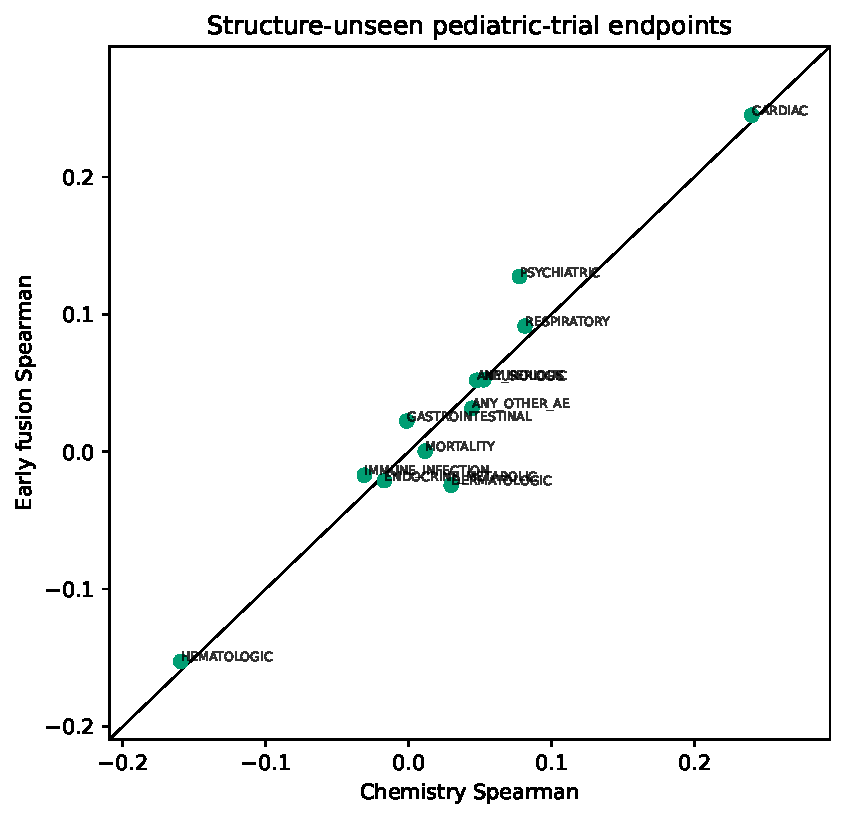
\includegraphics[width=0.88\linewidth]{figures/04_chem_vs_multimodal.pdf}
  \caption{Per-endpoint chemistry versus early fusion on the structure-unseen slice. Points near the diagonal are endpoints where the profile does not move the ranking.}
  \label{fig:chem}
\end{figure}

\begin{figure}[t]
  \centering
  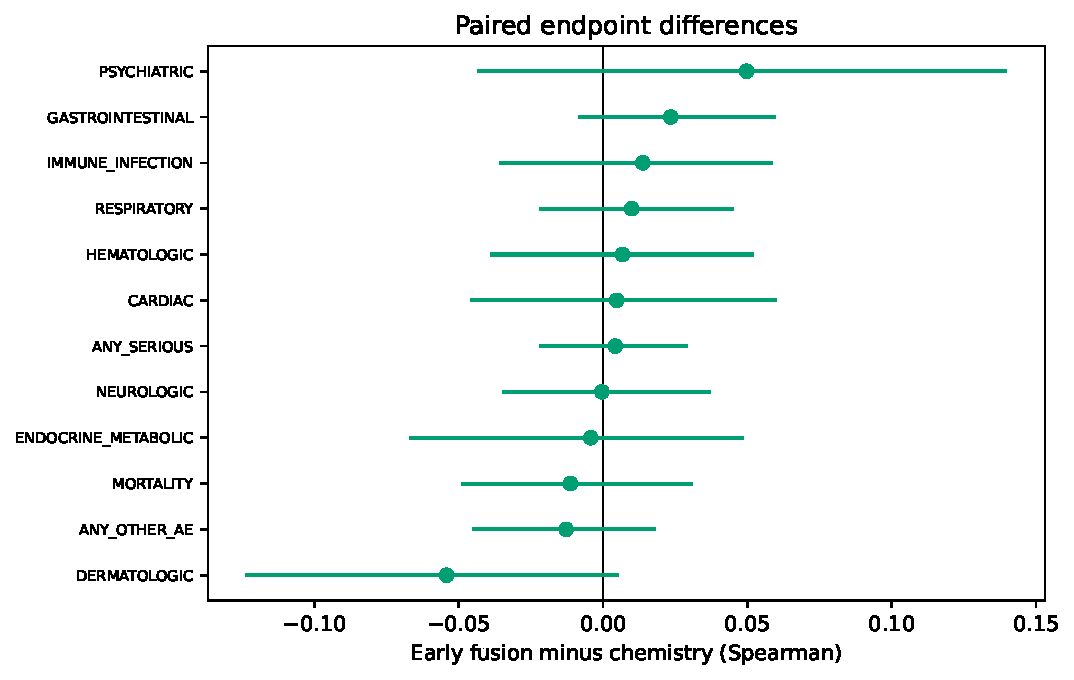
\includegraphics[width=0.92\linewidth]{figures/05_paired_differences.pdf}
  \caption{Endpoint-level early-fusion minus chemistry Spearman on the structure-unseen slice. The macro difference is the confirmatory estimand; several endpoints move in opposite directions.}
  \label{fig:paired}
\end{figure}

\section{Why the expected gain did not appear}
\label{sec:why}

\textbf{Reason for failure.}
Four facts, all computed from the saved predictions, account for the null without promoting a new primary test.

\textbf{The apparent signal is same-drug continuity.}
Table~\ref{tab:slices} decomposes the pediatric rows.
Chemistry's macro Spearman is $0.1923$ on structure-seen rows (mean $n$ per endpoint $404.6667$), $0.0314$ on structure-unseen rows (mean $n$ $109.6667$), and $0.1434$ on all pediatric rows (mean $n$ $514.3333$).
% src: results/tables/slice_macro.csv
Early fusion tracks chemistry on each of those slices ($0.1959$, $0.0339$, $0.1480$).
A pooled ``pediatric'' number mostly restates drugs the adult model has already seen.
Scaffold-unseen chemistry is $0.0180$ (mean $n$ $84.8333$), close to the structure-unseen result rather than to the seen-structure result.

\begin{table}[t]
\caption{Exploratory slice means for ridge Spearman. Structure-seen rows share an InChIKey with the adult trials. Coverage strata split the structure-unseen rows. Blank biology cells are undefined Spearman.}
\label{tab:slices}
\centering
\small
\begin{tabular}{lrrrr}
\toprule
Slice & Chem. & Early & Biology & Mean $n$ \\
\midrule
Structure-seen & $0.1923$ & $0.1959$ & $0.0837$ & $404.67$ \\
Structure-unseen & $0.0314$ & $0.0339$ & $0.0723$ & $109.67$ \\
All pediatric & $0.1434$ & $0.1480$ & $0.0766$ & $514.33$ \\
Unseen, any target & $0.2040$ & $0.1831$ & $0.1843$ & $24.00$ \\
Unseen, no target & $-0.0093$ & $-0.0081$ & --- & $85.67$ \\
\bottomrule
\end{tabular}
\end{table}
% src: results/tables/slice_macro.csv; mean n displayed to two decimals from the four-decimal table values 404.6667, 109.6667, 514.3333, 24.0000, 85.6667

\textbf{The biological channel is mostly missing.}
Mean missingness $0.9242$ means the gate is near zero for most compounds, so the gated prediction is nearly the chemical prediction (delta $-0.0007$).
Where any target is observed, mean $n$ is $24$ and chemistry ($0.2040$) is at least as high as early fusion ($0.1831$).
Where no target is observed, biology's Spearman is undefined because that block does not vary, and chemistry is $-0.0093$.
Missingness indicators alone have macro Spearman $0.0246$ ($95\%$ CI $-0.0381$ to $0.0821$), so the indicators are not a hidden label leak.
% src: results/tables/exploratory_intervals.csv spearman_missingness
Figure~\ref{fig:coverage} shows how thin the observed profile is.

\begin{figure}[t]
  \centering
  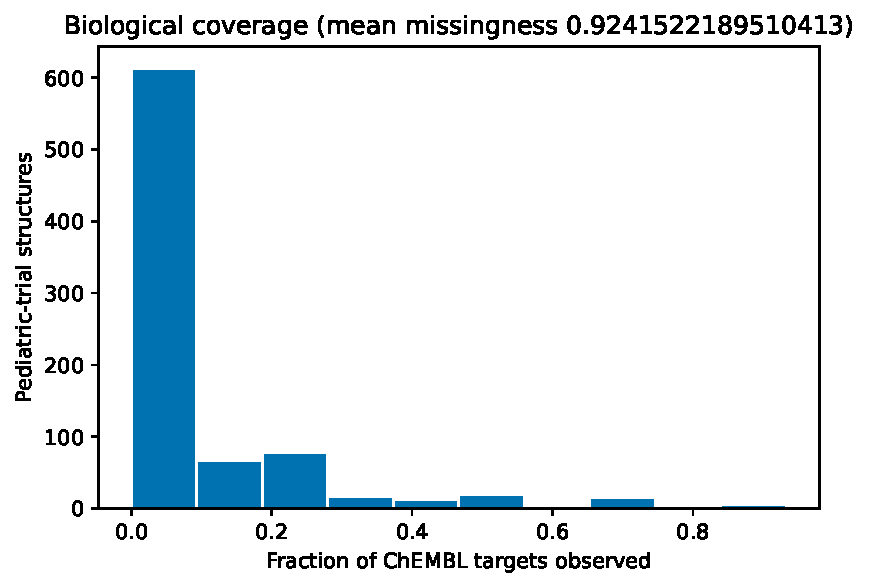
\includegraphics[width=0.86\linewidth]{figures/03_bio_coverage.pdf}
  \caption{Biological coverage on the trial structures. Most compounds have no observed ChEMBL target in this $15$-target vocabulary, so a coverage gate has little room to depart from chemistry.}
  \label{fig:coverage}
\end{figure}

\textbf{The chemical baseline is weak on the shift that matters.}
Adult scaffold Spearman $0.0220$ is detectably positive and practically small, and the structure-unseen chemistry interval includes $0$.
A fusion test on top of a near-null ranking has little headroom.
The adult macro RMSE of $3.0621$ on the logit scale is a second sign that the pre-specified penalty does not produce a sharp chemical score.
Because the penalty was not chosen on adult folds, this paper cannot say whether a different frozen penalty would move the point estimate.
It can say that the penalty was not chosen on the transfer test.

\textbf{The learned weight collapsed.}
The adult out-of-fold grid selected weight $1$ on early fusion.
Early and chemistry differ by $0.0004$ Spearman in that domain ($0.0224$ versus $0.0220$).
% src: results/tables/adult_indomain.csv ridge early 0.0224 and chem 0.0220
A validation rule with no source-domain gap cannot learn to ignore an unreliable channel.
Fixed $50/50$ mixtures and endpoint-wise weights land in the same narrow band as early fusion (macro Spearman $0.0330$ to $0.0345$ on the unseen slice).
% src: results/tables/transfer_macro.csv fixed_50_50_chem_bio 0.0345, fixed_50_50_chem_early 0.0335, late_endpoint_chem_early 0.0330
Random and permuted gates do as well ($0.0307$ and $0.0323$).
The non-deployable oracle, which looks at the label, reaches $0.0690$ and is only a ceiling.

Boundary conditions follow directly.
Do not read a multimodal null on a $15$-target, $92\%$ missing profile as a statement about biological representations in general.
Do not read a structure-seen Spearman near $0.19$ as evidence that the model generalized to new drugs.
Do not deploy the score as a clinical or regulatory safety tool.

\section{Lessons for multimodal biomedical transfer}
\label{sec:lessons}

Overlap audits come before transfer claims.
Here, $634$ of $835$ pediatric-trial structures are already in the adult table.
Removing them changes the chemical Spearman from $0.1434$ to $0.0314$.
Any benchmark that scores a ``new population'' without an identifier-level exclusion will credit continuity.

A reliability gate needs a source-domain signal to train against.
Weight collapse to pure fusion is a failure mode of validation-set mixing when the two source scores are interchangeable.
The gate then cannot protect the target.

Report the channel, not the word ``biology.''
Coverage, the fraction of compounds with any observation, and a missingness-only control belong next to the multimodal delta.
In this file those three numbers are $0.0758$, $0.3811$, and a contrast versus chemistry whose interval includes $0$ (missingness minus chemistry $-0.0068$, $95\%$ CI $-0.0747$ to $0.0739$).
% src: results/tables/exploratory_intervals.csv delta_missingness

Pre-register the family of tests.
Exploratory level intervals that exclude $0$ are easy to promote after the fact.
Biology-only and CORAL are in that category and are confined to the appendix.
They do not overturn Table~\ref{tab:primary}.

Name the label.
Trial incidence, spontaneous-report fractions, and assay hits answer different questions.
Mixing them produces an endpoint shift that no representation can honestly paper over.

\section{Follow-up: other fusions and a small network}
\label{sec:v5}

The three confirmatory tests use one ridge penalty and one early-fusion rule.
A later protocol, frozen before its own fits, asked whether a different combination rule or a small neural model would change the conclusion on the same twelve endpoints and the same structure-unseen InChIKeys.
That protocol is not part of the Benjamini--Hochberg family in Table~\ref{tab:primary}.
An arm in the follow-up is supported only if both of its $95\%$ endpoint-bootstrap intervals lie above $0$: the arm minus its matched chemistry model, and the arm minus the mean of the same arm under training-row permutations of biology, seeds $101$, $202$, $303$, $404$, and $505$.

The follow-up rebuilds chemistry from PubChem SMILES and the $15$ target values from the public ChEMBL API.
Mean missingness of that rebuilt profile is $0.9242$, on $3{,}057$ structures of which $201$ are structure-unseen.
% src: reports/v5_results.md rebuilt ChEMBL mean missingness 0.9242; structures 3057; unseen 201
These are not the original feature matrices, so the contrasts are against the matched rebuilt chemistry model, not against the confirmatory Spearman of $0.0314$.

Table~\ref{tab:v5} records the six arms.
None is supported.
The largest point estimate is a late stack of a ridge on Tox21 assay outcomes with chemistry, $0.0543$ ($95\%$ CI $-0.0291$ to $0.1333$).
The multitask network, one hidden layer of $64$ units trained on Morgan bits with and without the target block, is worse with the target block than without it ($-0.0167$, $95\%$ CI $-0.0401$ to $0.0079$).
Chemical Checker signatures, Chemprop, PyTorch Geometric, and pretrained embedding weights were not available and were not given a score.

\begin{table}[t]
\caption{Follow-up arms on the structure-unseen slice. Deltas are macro Spearman. Intervals are $1{,}000$ endpoint resamples. A supported arm would need both intervals above $0$.}
\label{tab:v5}
\centering
\small
\begin{tabular}{lrrrr}
\toprule
Arm & vs chem. & $95\%$ CI & vs perm. & $95\%$ CI \\
\midrule
Late stack & $0.0082$ & $-0.0014$, $0.0200$ & $0.0087$ & $-0.0010$, $0.0215$ \\
Missingness gate & $0.0021$ & $-0.0124$, $0.0200$ & $0.0017$ & $-0.0153$, $0.0201$ \\
Imputed targets & $-0.0016$ & $-0.0035$, $0.0001$ & $-0.0017$ & $-0.0035$, $0.0000$ \\
Targets, then label & $0.0444$ & $-0.0391$, $0.1170$ & $0.0151$ & $-0.0385$, $0.0625$ \\
Multitask network & $-0.0167$ & $-0.0401$, $0.0079$ & $-0.0013$ & $-0.0140$, $0.0092$ \\
Tox21-assay stack & $0.0543$ & $-0.0291$, $0.1333$ & $0.0651$ & $-0.0032$, $0.1363$ \\
\bottomrule
\end{tabular}
\end{table}
% src: reports/v5_results.md verdict lines; results/v5/primary_contrasts.csv

Two diagnostics sit outside that table.
A ridge on the rebuilt profile does not predict the frozen chemistry residual on adult out-of-fold rows (macro Spearman $-0.0143$).
% src: reports/v5_results.md residual macro mean -0.0143
Chemistry does predict the targets themselves: mean scaffold out-of-fold Spearman $0.2815$ across the $15$ targets.
% src: reports/v5_results.md redundancy mean 0.2815
The channel overlaps structure, and that overlap does not produce a gain on the trial label.
Replacing zero-filled targets with a training-set median moves an exploratory early ridge from $-0.0142$ to $-0.0081$.
% src: reports/v5_results.md zero-filled -0.0142; train-median -0.0081

\section{Limitations}
\label{sec:limits}

The structure-unseen sets are small, and the twelve endpoints are not independent.
The endpoint bootstrap matches the claim and is still a bootstrap of twelve numbers.
Forty-eight of the $201$ unseen structures share a scaffold with the source, so even the primary slice is not a pure scaffold holdout.
The ChEMBL release is unidentified, and the vocabulary was chosen by an earlier adult-coverage filter.
Chemical Checker signatures were not built.
The full nested-penalty config was not executed.
CORAL and importance weighting see unlabeled target chemistry; the target-only reference sees target labels.
Indication and reporting completeness remain inside the label.
Nothing here is a clinical decision rule.

\section*{Broader impact statement}

The positive use of this work is to separate same-drug continuity from generalization, and to name the endpoint as trial adverse-event incidence.
That can keep a Spearman near $0.19$ on overlapping structures from being described as pediatric toxicity performance.
The negative use is treating the scores as dosing, screening, or regulatory evidence.
On structures absent from the adult trials, the chemical rank correlation is compatible with zero, and the label is entangled with indication and reporting.
Structure-level predictions can also be misread as patient-level risk.
Mitigations are already in the protocol: the primary slice drops structures seen in adult trials, the claim requires intervals above zero, the ChEMBL matrix is not redistributed with the submission, and the text does not offer a clinical decision rule.
The aggregates are counts from a public trial registry, not patient records.

\section*{Reproducibility}

The confirmatory command is \texttt{python scripts/reproduce\_all.py --config configs/reduced.yaml}.
It refuses to start unless the analysis plan contains the frozen-protocol marker, which was committed before the fit.
The fit manifest records commit \texttt{a9324cf}, timestamp 2026-10-19T15:29:45Z, penalty mode prespecified, and the package versions used (Python $3.12.3$, scikit-learn $1.9.1$, RDKit $2026.9.1$, XGBoost $3.4.1$).
% src: results/run_manifest.json and results/tables/compute_runtime.csv
The trial prediction file has SHA-256 \texttt{37dbf42edac39337d9e76aeb446661dd7e3a0e16429d453cfd4d93abf68faa0d}.
Tables and figures for the confirmatory section are functions of that file.
The follow-up command is \texttt{python scripts/v5\_run.py}, which refuses to start unless \texttt{reports/v5\_preregistration.md} contains its frozen marker.
Its claims file is \texttt{results/v5/v5\_claims.json}.
The synthetic smoke config does not use the trial tables and does not update either claim.
The nested-penalty command was not the source of any number in Table~\ref{tab:primary}.
Anonymized code and the prediction files are the supplementary material.
This PDF does not link a repository or preprint that names the authors.

\section*{Use of large language models}

A large language model drafted the prose from the saved tables and the pre-registered plans.
It did not choose the eligibility cutoff, the penalty, the permutation seeds, or which contrasts were confirmatory.
Numerical sentences were checked against those tables.
The authors are responsible for the content, including the text drafted by the model.

\bibliographystyle{tmlr}
\bibliography{references}

\appendix

\section{Exploratory arms that are not confirmatory}
\label{app:explore}

Table~\ref{tab:explore} repeats endpoint-bootstrap intervals that were not in the Benjamini--Hochberg family.
Biology-only macro Spearman is $0.0723$ ($95\%$ CI $0.0042$ to $0.1441$).
Biology minus chemistry is $0.0409$ ($95\%$ CI $-0.0383$ to $0.1220$).
The second interval includes $0$.
CORAL chemistry is $0.0985$ ($95\%$ CI $0.0172$ to $0.1753$), and CORAL minus chemistry is $0.0671$ ($95\%$ CI $-0.0588$ to $0.1711$).
CORAL sees unlabeled pediatric features \citep{sun2016coral}.
Importance-weighted chemistry is $0.0239$ ($95\%$ CI $-0.0154$ to $0.0639$).
Early fusion without missingness indicators differs from chemistry by $0.0025$ ($95\%$ CI $-0.0041$ to $0.0100$).
A chemistry model trained on permuted adult labels scores $-0.0348$, which is a negative control rather than a transfer method.
% src: results/tables/transfer_macro.csv ridge chem_ylabel_permuted_seed_101

\begin{table}[h]
\caption{Exploratory endpoint-bootstrap intervals on the twelve eligible endpoints. Not adjusted with the three confirmatory tests.}
\label{tab:explore}
\centering
\small
\begin{tabular}{lrr}
\toprule
Quantity & Estimate & $95\%$ CI \\
\midrule
Biology only & $0.0723$ & $0.0042$, $0.1441$ \\
Biology minus chemistry & $0.0409$ & $-0.0383$, $0.1220$ \\
CORAL chemistry & $0.0985$ & $0.0172$, $0.1753$ \\
CORAL minus chemistry & $0.0671$ & $-0.0588$, $0.1711$ \\
Importance-weighted chemistry & $0.0239$ & $-0.0154$, $0.0639$ \\
Missingness only & $0.0246$ & $-0.0381$, $0.0821$ \\
\bottomrule
\end{tabular}
\end{table}
% src: results/tables/exploratory_intervals.csv

On a scaffold holdout that uses target labels for half of the structure-unseen compounds, ridge chemistry has macro Spearman $0.1211$ and early fusion $0.1166$.
% src: results/tables/target_reference.csv
That arm is a labeled reference, not a zero-shot transfer, and fusion does not win it.

Tree point estimates on the same unseen slice, without a pre-specified interval, are: random-forest chemistry $0.0548$ and early fusion $0.0244$; XGBoost chemistry $0.0050$ and early fusion $0.0552$.
% src: results/tables/transfer_macro.csv
The XGBoost gap was not a confirmatory test, adult out-of-fold predictions were not used to set its hyperparameters, and no interval was pre-registered.
It is reported so that it is not hidden.
It is not a claim that gradient boosting plus the profile succeeds.

Moderator correlations of the early-minus-chemistry delta with coverage ($-0.5324$), scaffold novelty ($0.5464$), adult chemistry Spearman ($-0.1119$), unseen $n$ ($-0.2312$), and mean label ($0.1748$) use twelve endpoints.
% src: results/tables/moderator_associations.csv
They are not causal effects.

Figure~\ref{fig:perm} compares true and permuted biological features.
The permutation seeds' chemistry-plus-biology macro Spearman values on the unseen slice are $0.0278$, $0.0284$, $0.0470$, $0.0212$, and $0.0296$ for seeds $101$, $202$, $303$, $404$, and $505$.
% src: results/tables/transfer_macro.csv ridge chem_permuted_bio_seed_*

\begin{figure}[h]
  \centering
  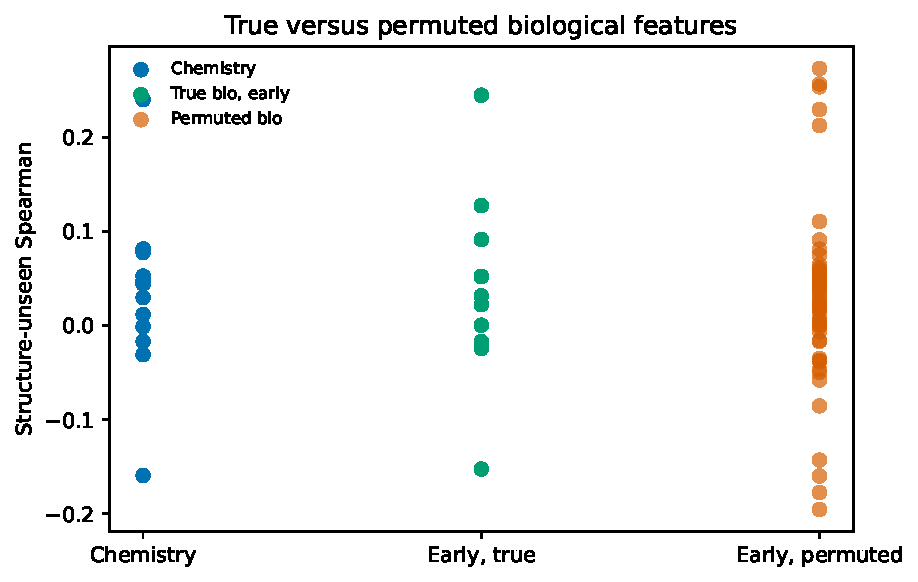
\includegraphics[width=0.92\linewidth]{figures/06_true_vs_permuted.pdf}
  \caption{True biological features versus training-row permutations. The confirmatory comparison is early fusion against the mean of these controls, not against a single seed.}
  \label{fig:perm}
\end{figure}

\section{Tox21 chemical baseline}
\label{app:tox21}

Tox21 is a separate in-vitro question \citep{wu2018moleculenet,tice2013tox21}.
The arm in this repository is logistic regression on Morgan fingerprints only, with scaffold GroupKFold and a shuffled $K$-fold, both with five splits.
It is not the archived XGBoost pipeline.
Biological signatures were not run.
Compounds: $7{,}587$.
Labels: $75{,}521$.
An assay is scored only with at least $20$ positives and $20$ negatives; all twelve tasks met that bar.
% src: reports/results.md Tox21 section and results/metrics/tox21_summary.json

Scaffold-split macro AUROC is $0.6895$ and macro AUPRC is $0.2440$.
Nuclear-receptor assays are $0.7034$ and stress-response assays are $0.6700$ under that split.
The random split, which allows scaffold leakage, has macro AUROC $0.7331$ and macro AUPRC $0.3200$.
The random-minus-scaffold gap is $0.0436$.
Nuclear receptor versus stress response is a comparison of assay families under one split, not a label-aligned transfer.
The gap shows that this chemical baseline does rank assay hits, and that a random split overstates that ranking.
It does not rescue the trial-incidence null.

The archived notebook number $0.8224$ versus $0.8254$ used XGBoost and, for the second figure, Chemical Checker spaces that this fit did not rebuild.
% src: reports/initial_audit.md
Those two AUROCs are not recomputed here.

\section{Endpoint deltas}
\label{app:endpoints}

Table~\ref{tab:endpoints} lists every eligible endpoint.
Signs disagree.
No endpoint was dropped after seeing its delta.
The three endpoints below the frozen count cutoff stay out of the mean.

\begin{table}[h]
\caption{Structure-unseen ridge Spearman by endpoint, early fusion minus chemistry. Sorted by the delta. All twelve rows enter the confirmatory macro.}
\label{tab:endpoints}
\centering
\small
\begin{tabular}{lrrrr}
\toprule
Endpoint & $n$ & Chem. & Early & Delta \\
\midrule
Dermatologic & $82$ & $0.0298$ & $-0.0243$ & $-0.0541$ \\
Any other adverse event & $200$ & $0.0443$ & $0.0316$ & $-0.0127$ \\
Mortality & $144$ & $0.0117$ & $0.0004$ & $-0.0113$ \\
Endocrine/metabolic & $72$ & $-0.0169$ & $-0.0211$ & $-0.0042$ \\
Neurologic & $106$ & $0.0526$ & $0.0523$ & $-0.0003$ \\
Any serious & $200$ & $0.0477$ & $0.0520$ & $0.0043$ \\
Cardiac & $49$ & $0.2402$ & $0.2449$ & $0.0047$ \\
Hematologic & $59$ & $-0.1594$ & $-0.1526$ & $0.0068$ \\
Respiratory & $107$ & $0.0815$ & $0.0915$ & $0.0100$ \\
Immune/infection & $113$ & $-0.0309$ & $-0.0171$ & $0.0138$ \\
Gastrointestinal & $120$ & $-0.0012$ & $0.0223$ & $0.0235$ \\
Psychiatric & $64$ & $0.0777$ & $0.1275$ & $0.0498$ \\
\bottomrule
\end{tabular}
\end{table}
% src: reports/results.md endpoint list, which matches results/statistics/endpoint_contrasts.csv

\section{Design schematic}
\label{app:design}

Figure~\ref{fig:design} is the analysis flow used to generate the predictions.
It does not add a numeric claim.

\begin{figure}[h]
  \centering
  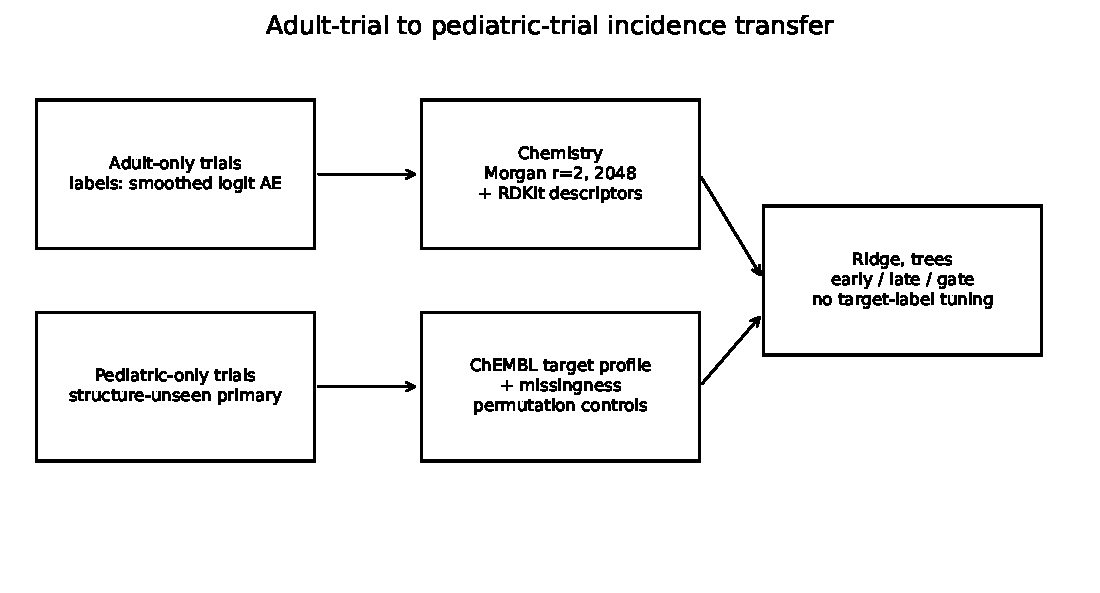
\includegraphics[width=0.95\linewidth]{figures/01_design_schematic.pdf}
  \caption{Flow from adult-trial fitting to the structure-unseen evaluation. Counts and metrics in the text are taken from the saved tables, not from this drawing.}
  \label{fig:design}
\end{figure}

\end{document}
